\section{Illustrative 6-node example.}
\label{app:illustration}

Let us consider the task graph of Figure~\ref{fig:demosoftmakespan}. The numerical values below are illustrative demo values used only to explain the differentiable soft scheduler.

\begin{figure}[!htbp]
\centering
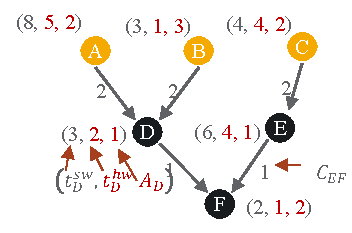
\includegraphics[width=0.52\linewidth]{Figures/methods/demosoftmakespan.pdf}
\caption{Illustrative 6-node fork-join task graph used to explain the differentiable soft scheduler. Each node is annotated with $(t_i^{sw}, t_i^{hw}, A_i)$ and each edge label denotes communication cost.}
\label{fig:demosoftmakespan}
\end{figure}

The graph has dependencies
\[
A \rightarrow D,\quad B \rightarrow D,\quad C \rightarrow E,\quad D \rightarrow F,\quad E \rightarrow F.
\]

For this example, the placement head predicts
\begin{equation}
\tilde{\vp}=[0.05,\,0.05,\,0.05,\,0.95,\,0.95,\,0.95]^\top,
\end{equation}
for tasks $(A,B,C,D,E,F)$, indicating that $A,B,C$ are nearly assigned to software, while $D,E,F$ are nearly assigned to hardware. The ordering head predicts
\begin{equation}
\tilde{\vpi}^{sw}=[0.00,\,-1.00,\,1.00,\,-0.50,\,-0.75,\,-0.25]^\top.
\end{equation}

Using the task costs in Figure~\ref{fig:demosoftmakespan}, the relaxed execution times are
\begin{align}
\tilde t_A &= 0.05\cdot 5 + 0.95\cdot 8 = 7.85, &
\tilde t_B &= 0.05\cdot 1 + 0.95\cdot 3 = 2.90, \\
\tilde t_C &= 0.05\cdot 4 + 0.95\cdot 4 = 4.00, &
\tilde t_D &= 0.95\cdot 2 + 0.05\cdot 3 = 2.05, \\
\tilde t_E &= 0.95\cdot 4 + 0.05\cdot 6 = 4.10, &
\tilde t_F &= 0.95\cdot 1 + 0.05\cdot 2 = 1.05.
\end{align}
Similarly, the soft communication on the cut edges is
\begin{equation}
\tilde c_{AD}=\tilde c_{BD}=\tilde c_{CE}=|0.05-0.95|\cdot 2 = 1.8,
\end{equation}
while $\tilde c_{DF}=\tilde c_{EF}=0$ because the corresponding communication cost is $0$.

\paragraph{\textbf{Step 1: ordering head \(\rightarrow\) Sinkhorn matrix \(\rightarrow\) expected ranks.}}
Using the score-to-position compatibility
\begin{equation}
L_{ai} = -\frac{(\tilde{\pi}_i^{sw}-u_a)^2}{\tau_o},
\qquad
u_a = 1-\frac{2a}{n-1},
\quad a=0,\ldots,n-1,
\end{equation}
Sinkhorn normalization yields the soft permutation matrix
\begingroup
\setlength{\arraycolsep}{3pt}
\begin{equation}
\scriptsize
\mP^{sw}\approx
\begin{bmatrix}
0.181 & 0.002 & 0.695 & 0.029 & 0.008 & 0.084\\
0.332 & 0.015 & 0.257 & 0.120 & 0.047 & 0.229\\
0.271 & 0.060 & 0.043 & 0.218 & 0.128 & 0.280\\
0.143 & 0.155 & 0.005 & 0.255 & 0.224 & 0.219\\
0.056 & 0.302 & 0.000 & 0.223 & 0.291 & 0.128\\
0.017 & 0.467 & 0.000 & 0.155 & 0.302 & 0.060
\end{bmatrix},
\end{equation}
\endgroup
where rows correspond to positions \(a=0,\ldots,5\) and columns correspond to tasks \((A,B,C,D,E,F)\).

The expected ranks are then
\begin{equation}
\tilde r_i=\sum_{a=0}^{n-1} a\,\mP^{sw}_{ai},
\end{equation}
which gives
\begin{equation}
\tilde{\vr}^{sw}\approx
[1.613,\;4.141,\;0.357,\;2.986,\;3.649,\;2.258]^\top.
\end{equation}
Hence the induced global soft order is
\[
C \prec A \prec F \prec D \prec E \prec B,
\]
and the induced software order over the three nearly-software tasks is
\[
C \prec A \prec B.
\]

\paragraph{\textbf{Step 2: expected ranks \(\rightarrow\) before matrix.}}
Using the rank-sigmoid approximation,
\begin{equation}
B^{sw}_{ji}
=
\sigma\!\left(\frac{\tilde r_i-\tilde r_j}{\tau_r}\right),
\qquad
B^{sw}_{ii}=0,
\end{equation}
we obtain the soft before matrix
\begingroup
\setlength{\arraycolsep}{3pt}
\begin{equation}
\scriptsize
\mB^{sw}\approx
\begin{bmatrix}
0     & 0.999 & 0.027 & 0.981 & 0.997 & 0.863\\
0.001 & 0     & 0     & 0.036 & 0.197 & 0.005\\
0.973 & 1.000 & 0     & 0.999 & 1.000 & 0.996\\
0.019 & 0.964 & 0.001 & 0     & 0.869 & 0.111\\
0.003 & 0.803 & 0     & 0.131 & 0     & 0.018\\
0.137 & 0.995 & 0.004 & 0.889 & 0.982 & 0
\end{bmatrix},
\end{equation}
\endgroup
so, for example,
\[
B^{sw}_{CA}=0.973,\qquad B^{sw}_{CB}=1.000,\qquad B^{sw}_{AB}=0.999,
\]
which strongly supports the order \(C \prec A \prec B\).

\paragraph{\textbf{Step 3: gate using placement probabilities.}}
Since ordering matters only when both tasks are likely to execute in software, we use the gate
\begin{equation}
\mG^{sw}=(1-\tilde{\vp})(1-\tilde{\vp})^\top
=
\begin{bmatrix}
0.9025\,\mathbf{1}_{3\times 3} & 0.0475\,\mathbf{1}_{3\times 3}\\
0.0475\,\mathbf{1}_{3\times 3} & 0.0025\,\mathbf{1}_{3\times 3}
\end{bmatrix},
\end{equation}
because \(1-\tilde p_i=0.95\) for \(A,B,C\) and \(1-\tilde p_i=0.05\) for \(D,E,F\).

The effective resource-order matrix is
\begin{equation}
\mR^{sw}=\mB^{sw}\odot \mG^{sw},
\end{equation}
which gives
\begingroup
\setlength{\arraycolsep}{3pt}
\begin{equation}
\scriptsize
\mR^{sw}\approx
\begin{bmatrix}
0     & 0.902 & 0.024 & 0.047 & 0.047 & 0.041\\
0.001 & 0     & 0     & 0.002 & 0.009 & 0    \\
0.878 & 0.902 & 0     & 0.047 & 0.047 & 0.047\\
0.001 & 0.046 & 0     & 0     & 0.002 & 0    \\
0     & 0.038 & 0     & 0     & 0     & 0    \\
0.006 & 0.047 & 0     & 0.002 & 0.002 & 0
\end{bmatrix}.
\end{equation}
\endgroup
In particular,
\[
R^{sw}_{AB}=0.902,\qquad
R^{sw}_{CA}=0.878,\qquad
R^{sw}_{CB}=0.902,
\]
which strongly prefers \(C\) before \(A\) and \(B\), and \(A\) before \(B\).

\paragraph{\textbf{Step 4: DAG readiness and software readiness.}}
To make the effect concrete, we use the hard-order interpretation induced by the soft ranks. For the nearly-software tasks \(A,B,C\), the DAG-readiness values are
\[
s_A^{dag}=s_B^{dag}=s_C^{dag}=0,
\]
since they are source nodes. Thus, their ordering is driven entirely by the software-readiness term. Under the induced software order \(C\prec A\prec B\), we obtain approximately
\begin{align}
s_C^{sw} &\approx 0, &
\tilde s_C &\approx \max(s_C^{dag},s_C^{sw}) = 0, &
\tilde f_C &\approx 0 + 4.00 = 4.00,\\
s_A^{sw} &\approx \tilde f_C = 4.00, &
\tilde s_A &\approx \max(0,4.00) = 4.00, &
\tilde f_A &\approx 4.00 + 7.85 = 11.85,\\
s_B^{sw} &\approx \tilde f_A = 11.85, &
\tilde s_B &\approx \max(0,11.85) = 11.85, &
\tilde f_B &\approx 11.85 + 2.90 = 14.75.
\end{align}

Now consider the hardware tasks. Since \(D\) depends on both \(A\) and \(B\),
\begin{equation}
s_D^{dag}\approx \max(\tilde f_A+\tilde c_{AD},\,\tilde f_B+\tilde c_{BD})
=
\max(11.85+1.8,\;14.75+1.8)
=
16.55,
\end{equation}
and \(s_D^{sw}\approx 0\), so
\[
\tilde s_D\approx 16.55,\qquad
\tilde f_D\approx 16.55+2.05=18.60.
\]
Similarly, since \(E\) depends on \(C\),
\begin{equation}
s_E^{dag}\approx \tilde f_C+\tilde c_{CE}=4.00+1.8=5.80,
\end{equation}
hence
\[
\tilde s_E\approx 5.80,\qquad
\tilde f_E\approx 5.80+4.10=9.90.
\]
Finally, \(F\) depends on both \(D\) and \(E\), so
\begin{equation}
s_F^{dag}\approx \max(\tilde f_D,\tilde f_E)=\max(18.60,9.90)=18.60,
\end{equation}
which yields
\[
\tilde s_F\approx 18.60,\qquad
\tilde f_F\approx 18.60+1.05=19.65.
\]
Thus, the induced relaxed makespan is approximately
\[
L_{\mathrm{soft\mbox{-}makespan}} \approx 19.65.
\]

\paragraph{\textbf{Why \(C\prec A\prec B\) is better than \(A\prec B\prec C\).}}
If the software order were instead \(A\prec B\prec C\), then the same hard-order approximation gives
\[
\tilde f_A\approx 7.85,\qquad
\tilde f_B\approx 10.75,\qquad
\tilde f_C\approx 14.75.
\]
Therefore,
\[
s_D^{dag}\approx \max(7.85+1.8,\;10.75+1.8)=12.55,
\qquad
\tilde f_D\approx 14.60,
\]
while
\[
s_E^{dag}\approx 14.75+1.8=16.55,
\qquad
\tilde f_E\approx 20.65.
\]
This delays the \(C\rightarrow E\rightarrow F\) branch, and hence
\[
s_F^{dag}\approx \max(14.60,\;20.65)=20.65,
\qquad
\tilde f_F\approx 21.70.
\]
Thus,
\[
\mathrm{makespan}(C\prec A\prec B)\approx 19.65
\;<\;
\mathrm{makespan}(A\prec B\prec C)\approx 21.70.
\]

The reason is that the \(C\rightarrow E\) branch is the slower downstream branch: once \(C\) finishes, task \(E\) still needs about \(4.10\) units to complete, whereas the \(A,B\rightarrow D\) branch needs only about \(2.05\) units after both \(A\) and \(B\) finish. Prioritizing \(C\) earlier therefore reduces the final critical path.

\paragraph{\textbf{Why DAG-only readiness is insufficient.}}
Without the ordering head, a scheduler based only on DAG readiness cannot distinguish among the ready source tasks \(A,B,C\), because all three have
\[
s_A^{dag}=s_B^{dag}=s_C^{dag}=0.
\]
Any topological order, such as \(A\prec B\prec C\) or \(C\prec A\prec B\), is valid from the precedence perspective alone. However, these orders produce different software serialization patterns and different makespans. The ordering head resolves this ambiguity by producing a structured pairwise precedence matrix, which allows the soft scheduler to model resource-induced serialization in addition to DAG constraints.